\newpage
\section*{FIGURES}

\begin{figure}[!htbp]
    \centering
    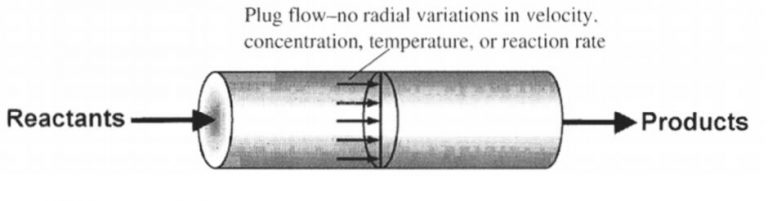
\includegraphics[width=0.7\textwidth]{Figures/sample.jpeg}
    \caption{Sample figure.}
    \label{fig:reactor_scheme}
\end{figure}

\begin{figure}[!htbp]
    \centering
    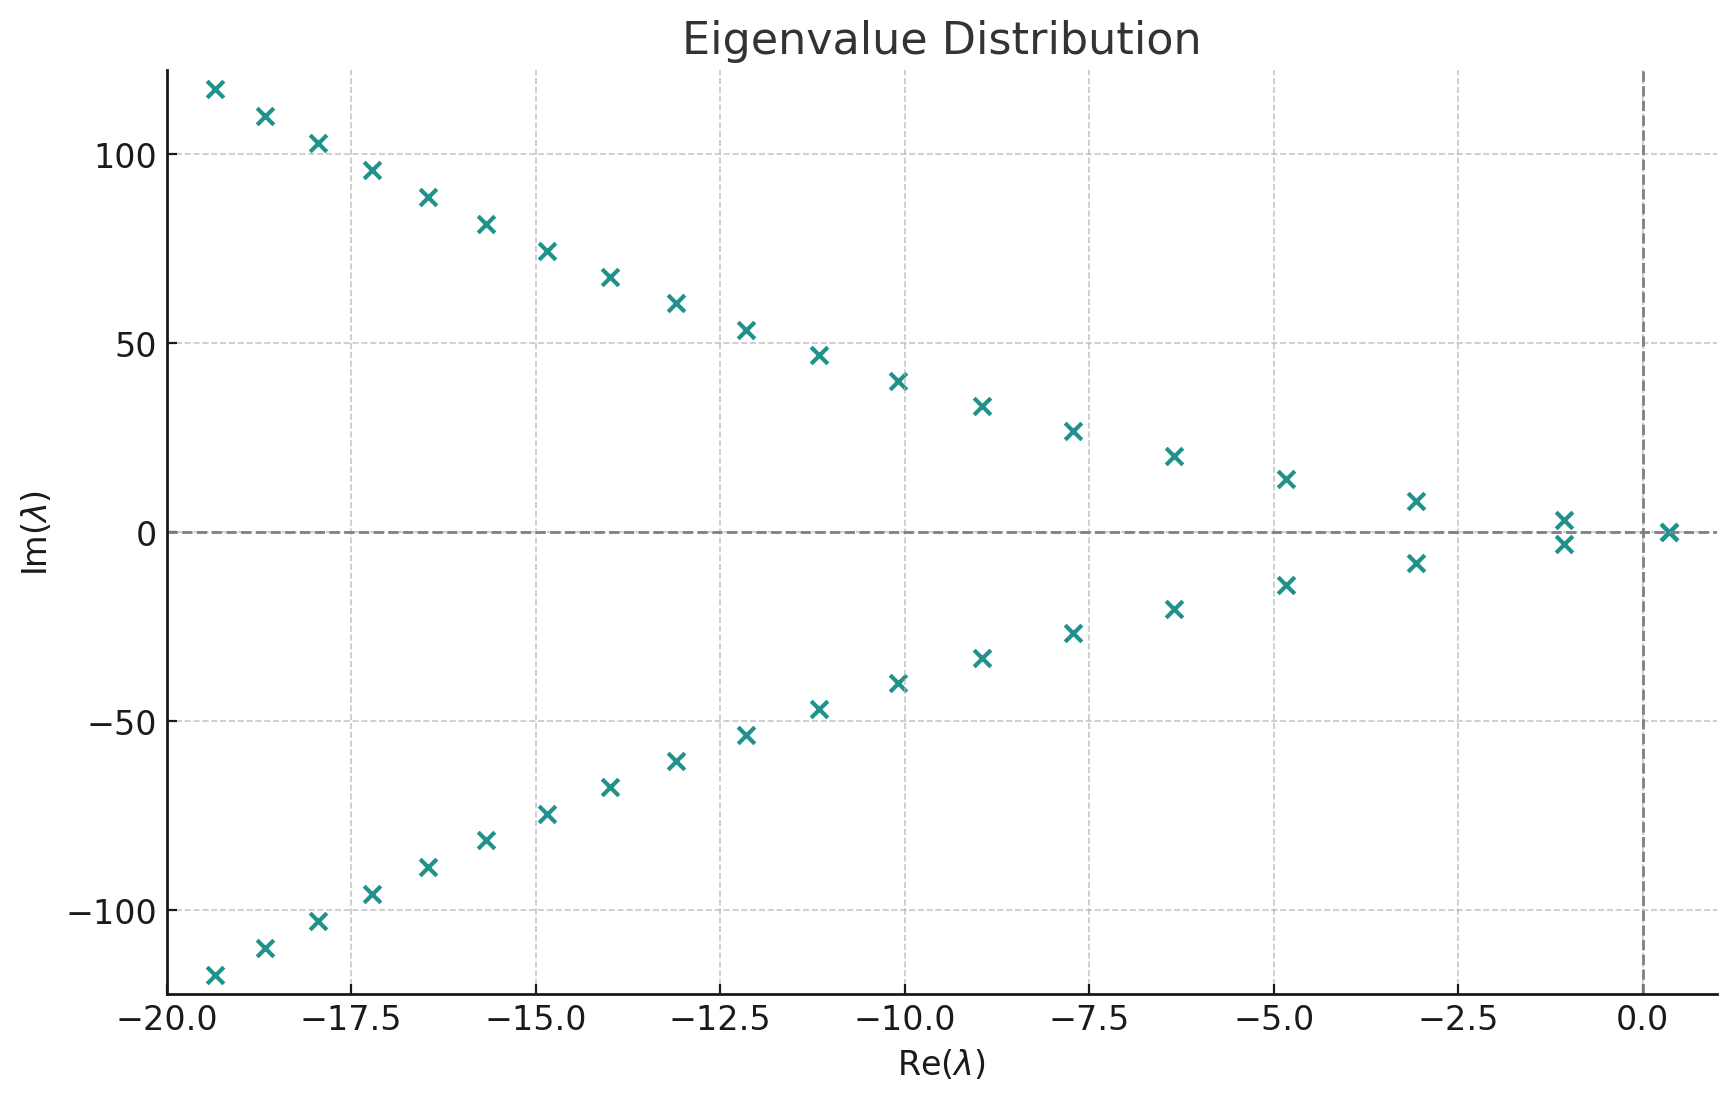
\includegraphics[width=0.7\textwidth]{Figures/eigval_dist_R_0.3.jpg}
    \caption{Eigenvalues of operator $\mathfrak{A}$ plotted on complex plane}
    \label{fig:eigval_dist}
\end{figure}

\begin{figure}[!htbp]
    \centering
    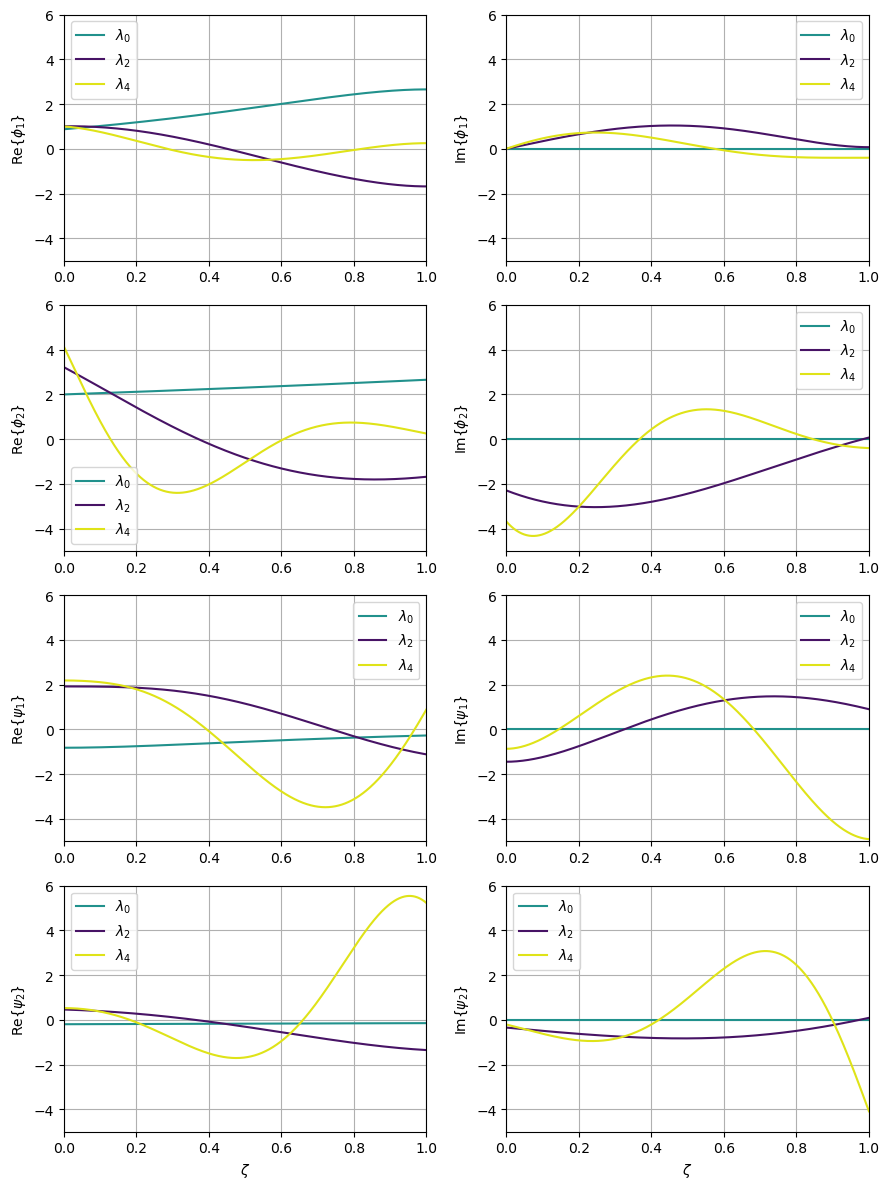
\includegraphics[width=0.7\textwidth]{Figures/eigfuns.png}
    \caption{First few eigenmodes of $\mathfrak{A}$ and $\mathfrak{A}^*$}
    \label{fig:eigfun}
\end{figure}

\begin{figure}[!htbp]
    \centering
    \begin{subfigure}[b]{0.45\textwidth}
        \centering
        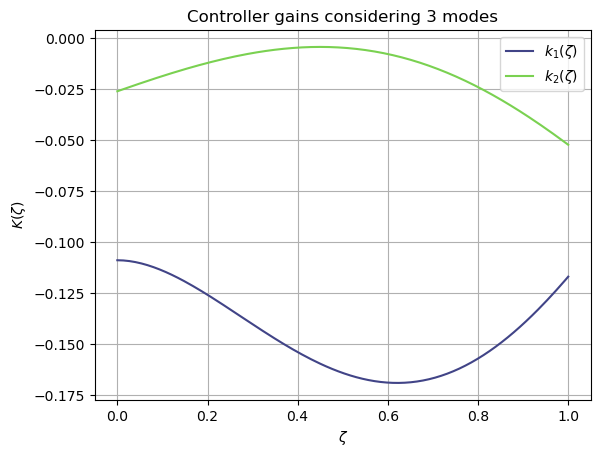
\includegraphics[width=\textwidth]{Figures/k_3.png}
        \caption{$N = 3$}
        \label{fig:k_3}
    \end{subfigure}
    \hfill
    \begin{subfigure}[b]{0.45\textwidth}
        \centering
        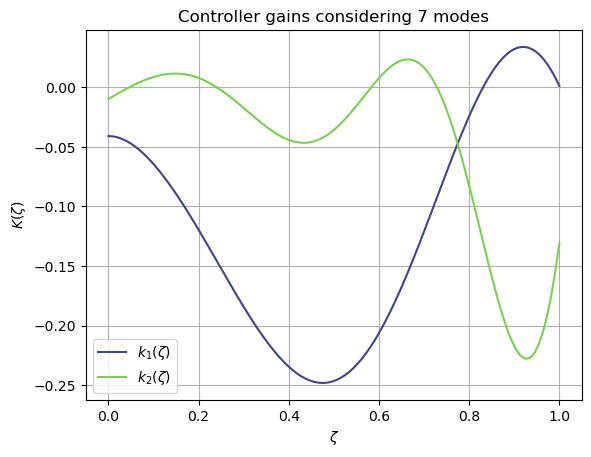
\includegraphics[width=\textwidth]{Figures/k_7.png}
        \caption{$N = 7$}
        \label{fig:k_7}
    \end{subfigure}
    \caption{Full-state feedback gain $K(\zeta)$ utilizing the first 7 modes of the system.}
    \label{fig:k_modes}
\end{figure}

\begin{figure}[!htbp]
    \centering
    \includegraphics*[width=0.7\textwidth]{Figures/sample.jpeg}
    \caption{Block diagram representation of the full-state feedback control system.}
    \label{fig:block_diagram}
\end{figure}

\begin{figure}[!htbp]
    \centering
    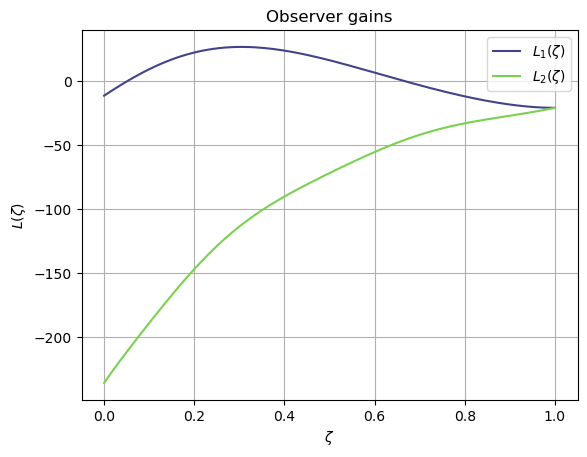
\includegraphics[width=0.7\textwidth]{Figures/L.png}
    \caption{Observer gain $L(\zeta)$.}
    \label{fig:L_modes}
\end{figure}

\begin{figure}[!htbp]
    \centering
    \includegraphics*[width=0.7\textwidth]{Figures/pole_placement.png}
    \caption{Eigenvalues of the observer-based controller, full-state feedback controller, and open-loop system.}
    \label{fig:eigs}
\end{figure}

\begin{figure}[!htbp]
    \centering
    \includegraphics*[width=0.7\textwidth]{Figures/sample.jpeg}
    \caption{Block diagram representation of the full-state feedback control system.}
    \label{fig:block_diagram_observer}
\end{figure}

\begin{figure}[!htbp]
    \centering
    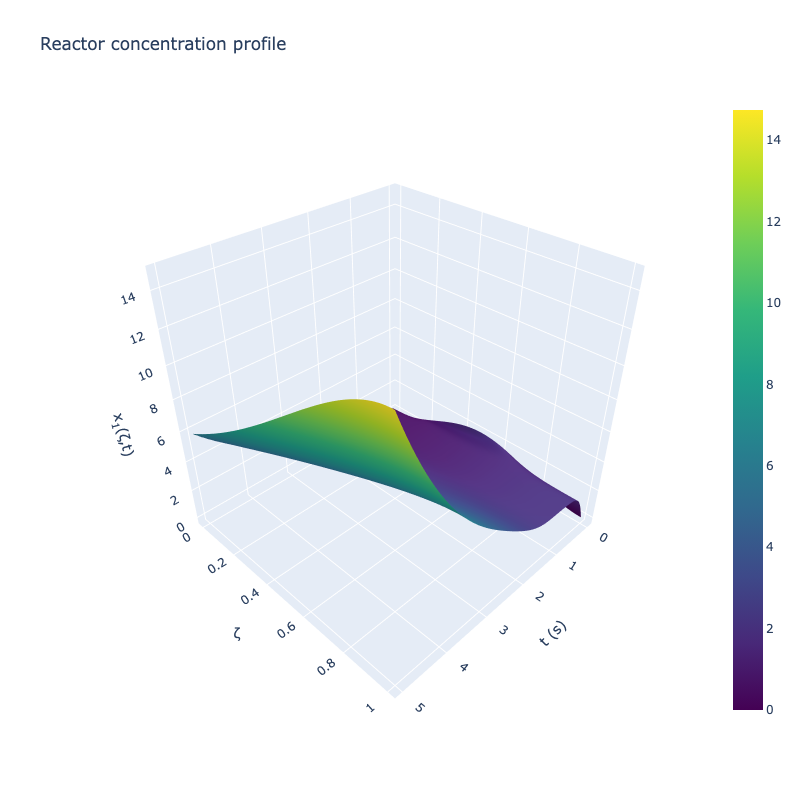
\includegraphics[width=0.8\textwidth]{Figures/3D_x1_openloop.png}
    \caption{3D plot of the open-loop system}
    \label{fig:3D_x1_openloop}
\end{figure}

\begin{figure}[!htbp]
    \centering
    \begin{subfigure}[b]{0.45\textwidth}
        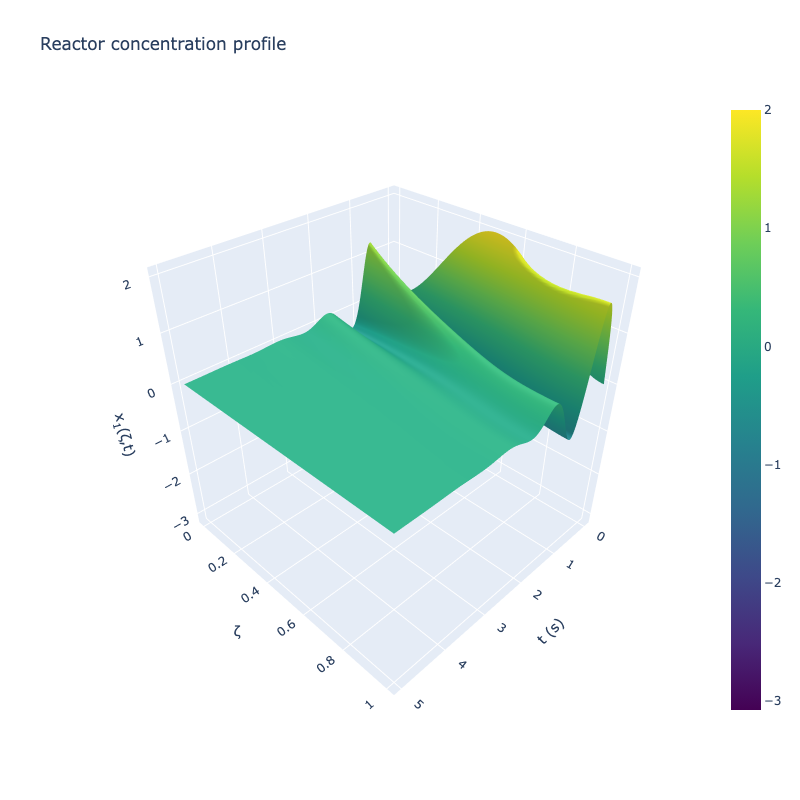
\includegraphics[width=\textwidth]{Figures/3D_x1_k3.png}
        \caption{Full-state feedback regulator with $N=3$}
        \label{fig:3D_x1_k3}
    \end{subfigure}
    \hfill
    \begin{subfigure}[b]{0.45\textwidth}
        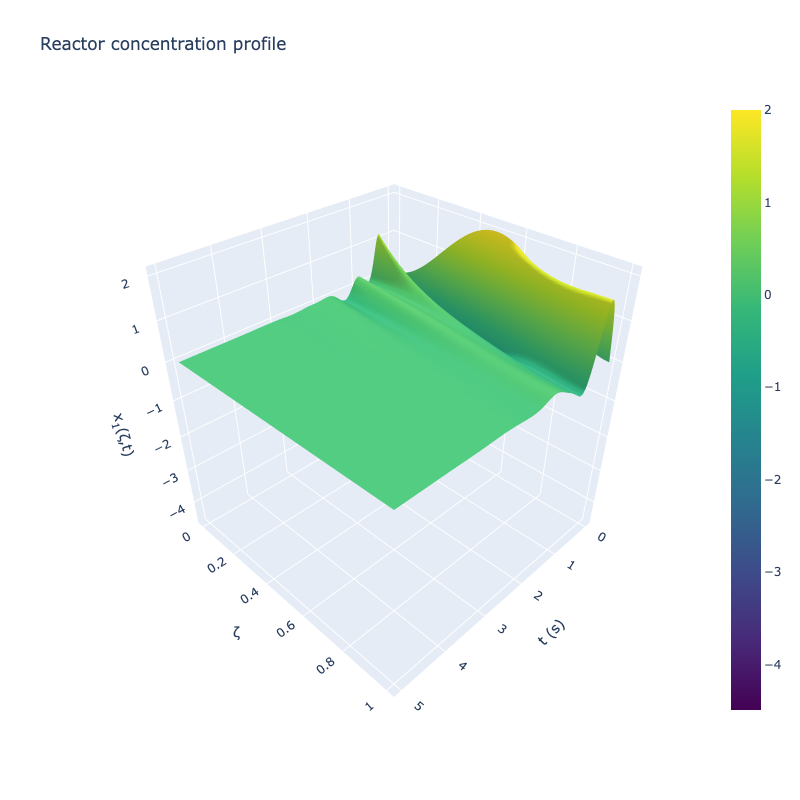
\includegraphics[width=\textwidth]{Figures/3D_x1_k7.png}
        \caption{Full-state feedback regulator with $N=7$}
        \label{fig:3D_x1_k7}
    \end{subfigure}
    \caption{FDM representation of the full-state feedback regulator}
    \label{fig:full_state_feedback}
\end{figure}

\begin{figure}[!htbp]
    \centering
    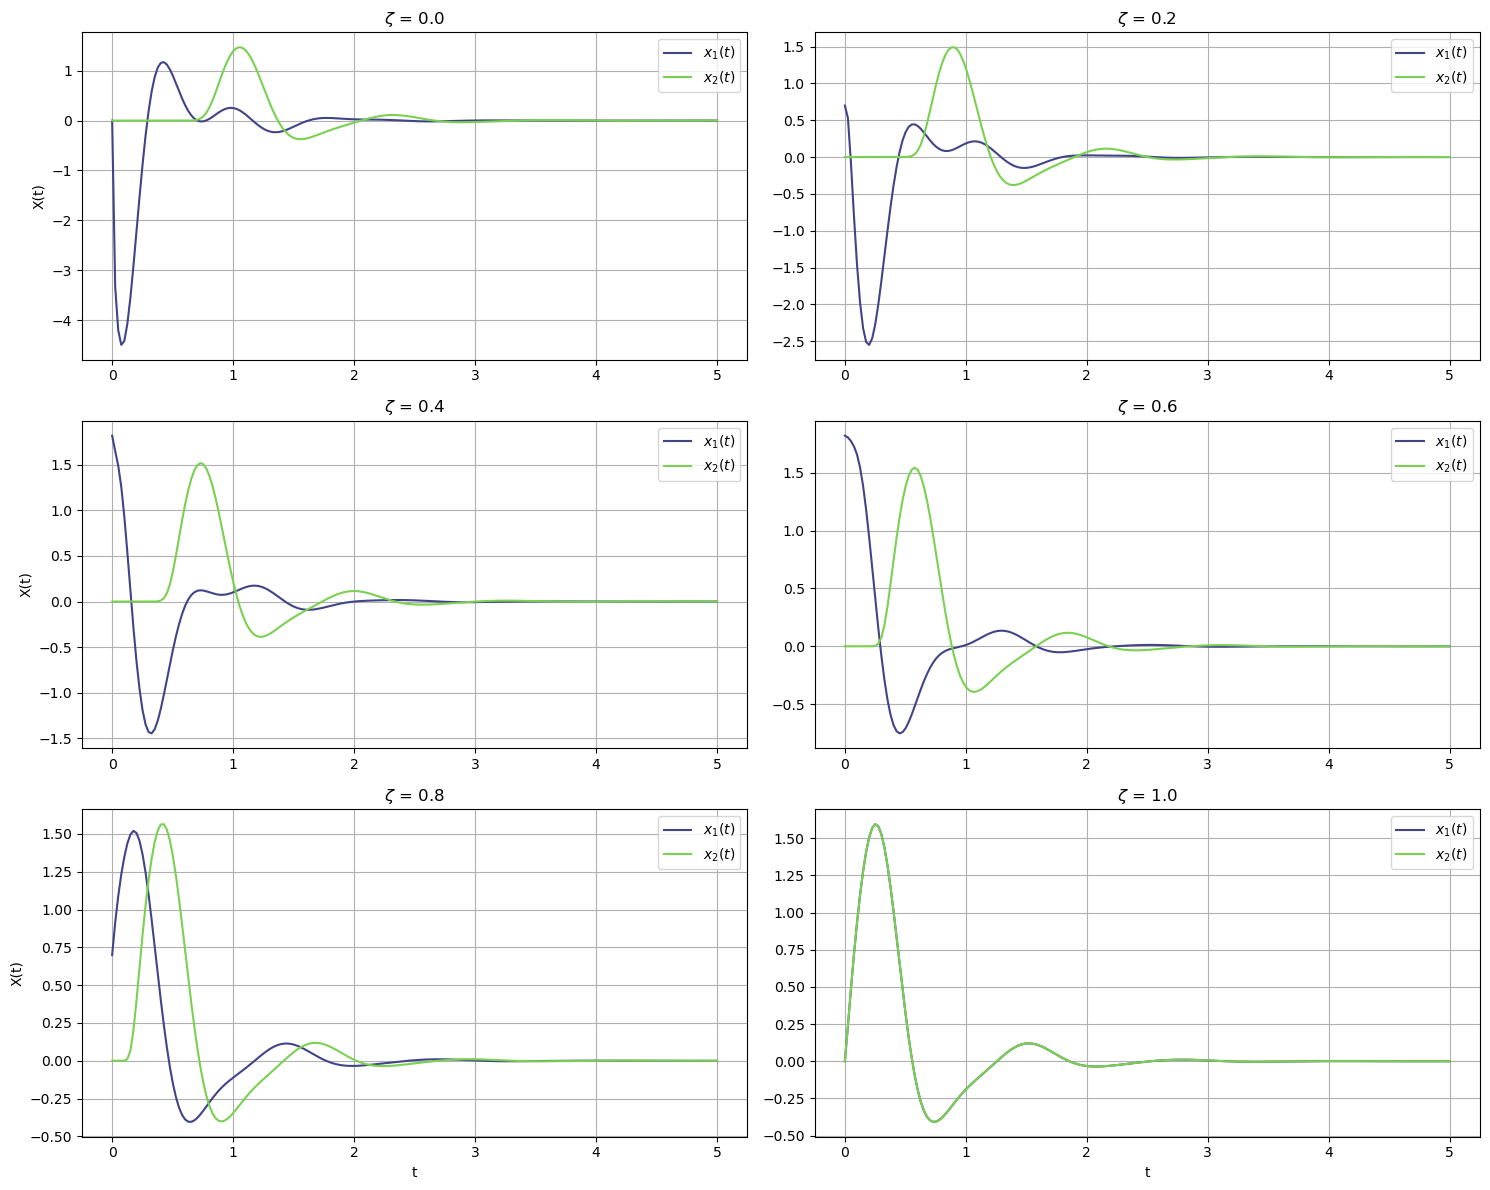
\includegraphics[width=0.8\textwidth]{Figures/2D_xt_k7.png}
    \caption{2D plot of the full-state feedback regulator with $N=7$}
    \label{fig:2D_xt_k7}
\end{figure}

\begin{figure}[!htbp]
    \centering
    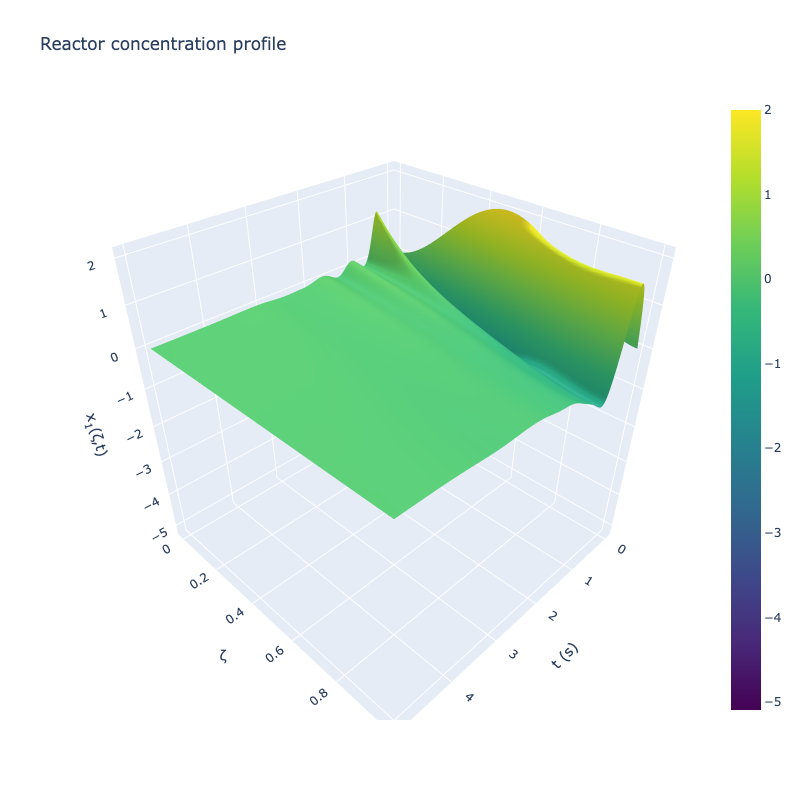
\includegraphics[width=0.8\textwidth]{Figures/3D_x1_L_k7.png}
    \caption{3D plot of the observer-based regulator}
    \label{fig:3D_x1_L_k7}
\end{figure}

\begin{figure}[!htbp]
    \centering
    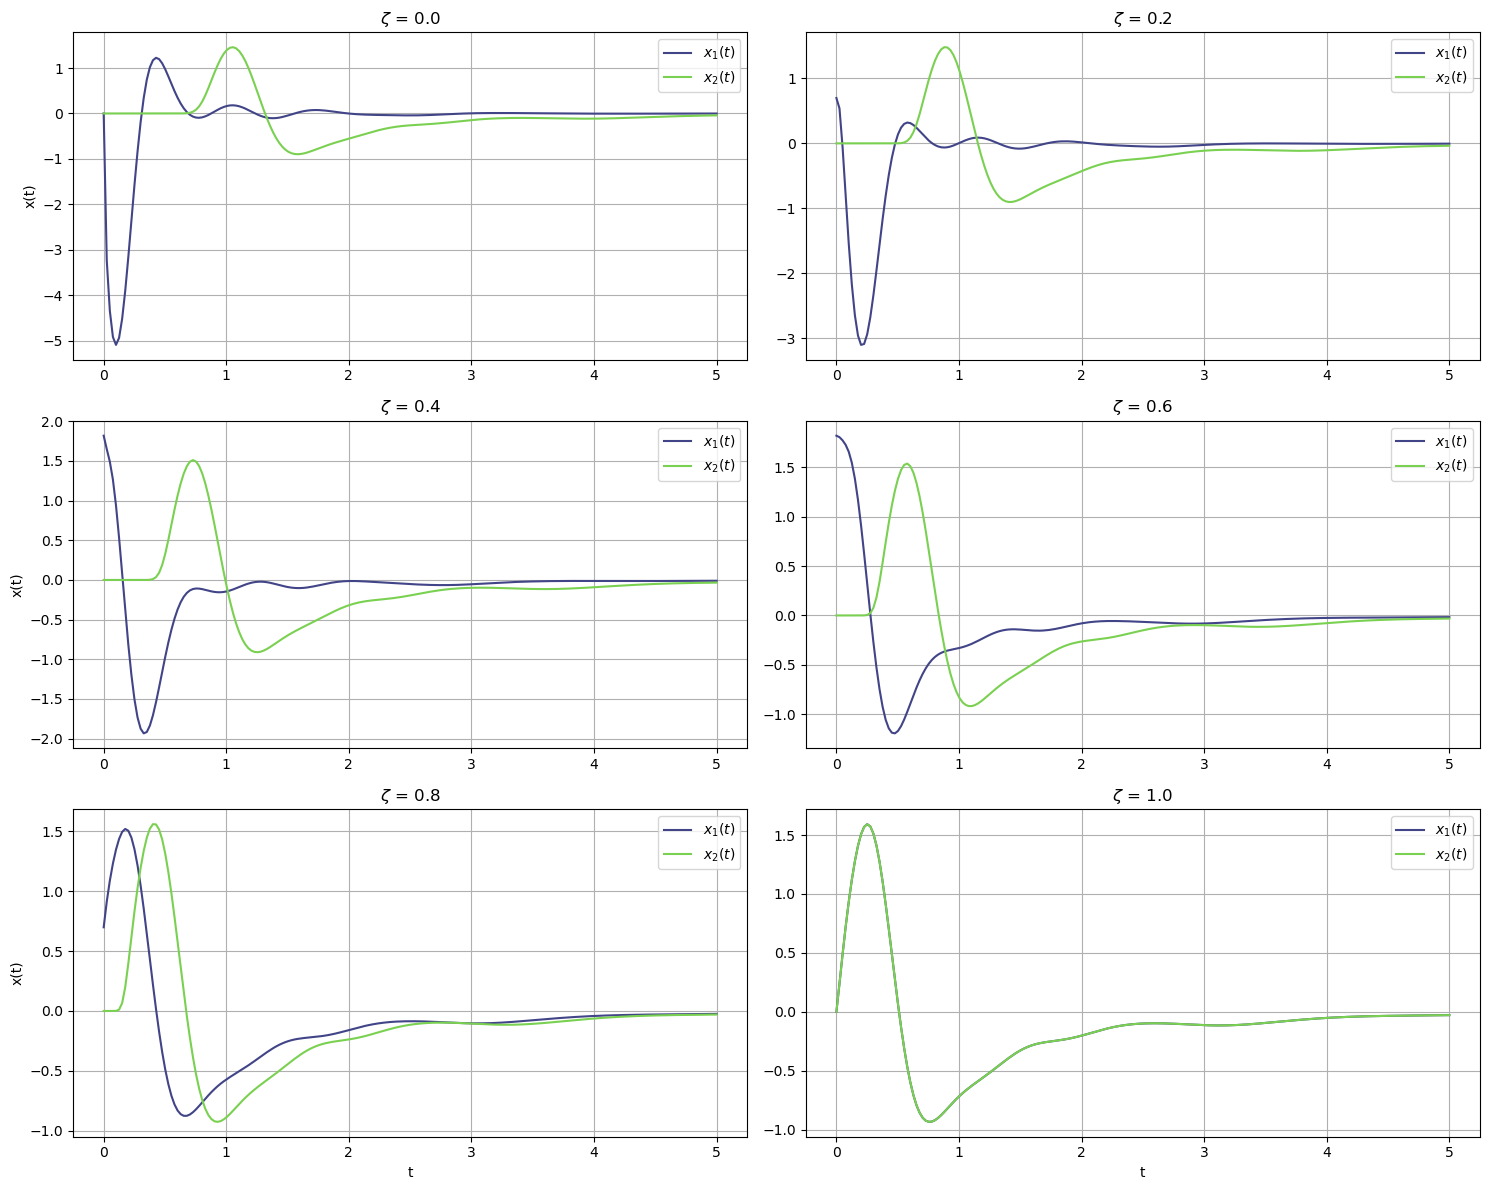
\includegraphics[width=0.8\textwidth]{Figures/2D_xt_L_k7.png}
    \caption{2D plot of the observer-based regulator}
    \label{fig:2D_xt_L_k7}
\end{figure}

\begin{figure}[!htbp]
    \centering
    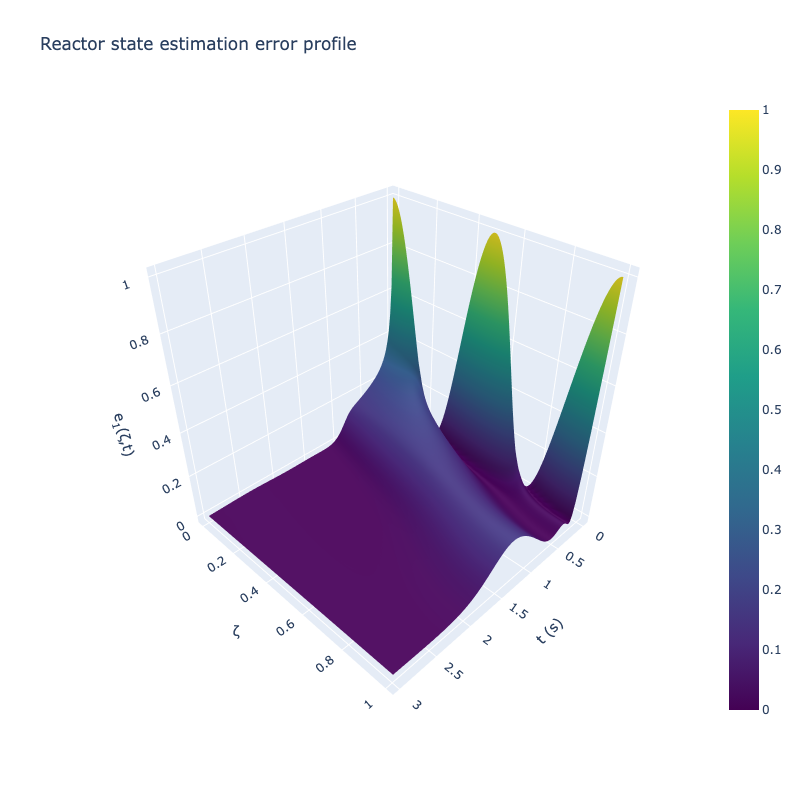
\includegraphics[width=0.8\textwidth]{Figures/3D_e1_L_k7.png}
    \caption{3D plot of the error dynamics of the observer-based regulator}
    \label{fig:3D_e1_L_k7}
\end{figure}

\begin{figure}[!htbp]
    \centering
    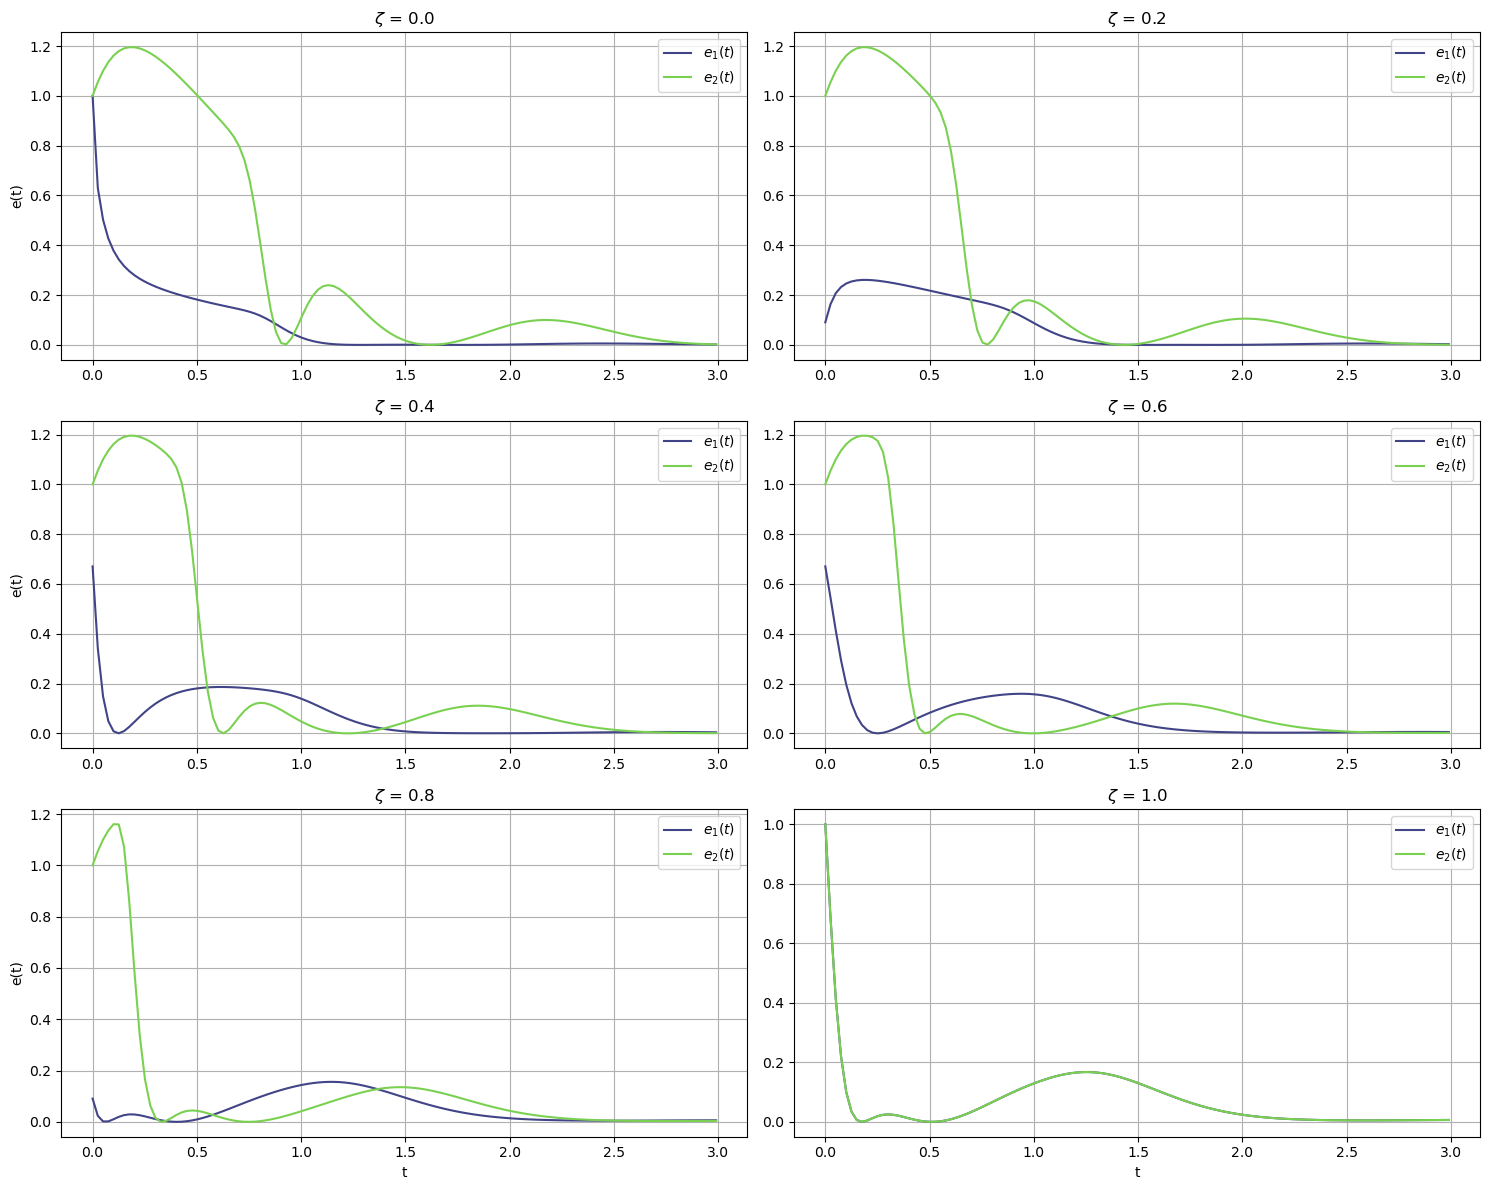
\includegraphics[width=0.8\textwidth]{Figures/2D_et_L_k7.png}
    \caption{2D plot of the error dynamics of the observer-based regulator}
    \label{fig:2D_et_L_k7}
\end{figure}
